\documentclass[11pt]{beamer}

% Required packages
\usepackage{booktabs}

\usepackage[siunitx]{circuitikz} 
% Theme settings
\usetheme{Boadilla}
\useinnertheme{circles}
\useoutertheme{miniframes}
\setbeamertemplate{navigation symbols}{}
\usepackage{ragged2e}
% Colors
\definecolor{primaryColor}{RGB}{126,36,150}
\definecolor{secondaryColor}{RGB}{175,50,209}

\usetikzlibrary{arrows.meta, positioning}
\setbeamercolor{structure}{fg=primaryColor}
\setbeamercolor{palette primary}{bg=primaryColor, fg=white}
\setbeamercolor{palette secondary}{bg=secondaryColor, fg=white}
\setbeamercolor{title}{bg=primaryColor, fg=white}
\setbeamercolor{headline}{bg=secondaryColor, fg=white}
\setbeamercolor{section in head/foot}{bg=primaryColor, fg=white}
\setbeamercolor{subsection in head/foot}{bg=secondaryColor, fg=white}
\setbeamercolor{author in head/foot}{bg=primaryColor, fg=white}
\setbeamercolor{title in head/foot}{bg=secondaryColor, fg=white}
\setbeamercolor{date in head/foot}{bg=primaryColor, fg=white}
\setbeamercolor{page number in head/foot}{bg=primaryColor, fg=white}

% Presentation metadata
\title[EN2130 Communication Design Project]{Two-Way Digital Paging System Using Software
	Defined Radios}
\author[BellLabz]{Ratnayake R.M.S.H.(230548R)\\
	Tennakoon U.G.R.B.(230629R)\\
	Disssanayake R.K.T.(230164K)\\
	Shehan M.N.N.(230613M)}
\institute[]{Department of Electronic \& Telecommunication Engineering\\ University of Moratuwa, Sri Lanka}
\date{\today}

% Document starts here
\begin{document}
	
	\begin{frame}
		\titlepage
	\end{frame}
	
	\begin{frame}
		\frametitle{Presentation Structure}
		\tableofcontents
	\end{frame}
	
	\section{Introduction}
	\begin{frame}{Abstraction}
		
\justifying
This project is a comprehensive \textbf{Software-Defined Radio (SDR)} platform that implements a complete digital communication protocol stack. The system integrates \textbf{QPSK physical layer transmission}, \textbf{Go-Back-N ARQ} for reliable data transfer, and \textbf{AES-128 encryption} for secure communications through intuitive user interfaces. By combining advanced signal processing algorithms with modern protocol design, this project demonstrates a \textbf{full-stack approach} that spans from physical layer processing to application-level messaging, making sophisticated telecommunications concepts accessible and operable in real-world scenarios.
	
	\end{frame}
	\begin{frame}{Block Diagram}
\begin{figure}[h]
	\centering
	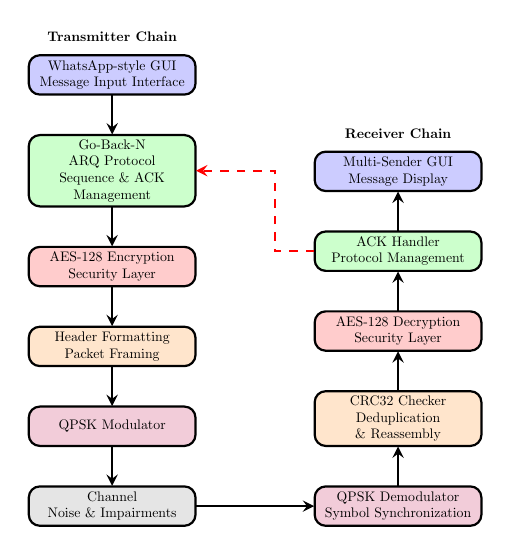
\begin{tikzpicture}[
		block/.style={rectangle, draw=black, thick, text width=4cm, minimum height=1cm, text centered, rounded corners},
		arrow/.style={->, thick, >=stealth},
		label/.style={text width=3cm, text centered}, transform shape, scale=0.5
		]
		
		% Transmitter Chain
		\node[block, fill=blue!20] (gui) {WhatsApp-style GUI \\ Message Input Interface};
		\node[block, fill=green!20, below=1cm of gui] (arq) {Go-Back-N ARQ Protocol \\ Sequence \& ACK Management};
		\node[block, fill=red!20, below=1cm of arq] (crypto) {AES-128 Encryption \\ Security Layer};
		\node[block, fill=orange!20, below=1cm of crypto] (header) {Header Formatting \\ Packet Framing};
		\node[block, fill=purple!20, below=1cm of header] (modulator) {QPSK Modulator};
		\node[block, fill=gray!20, below=1cm of modulator] (channel) {Channel \\ Noise \& Impairments};
		
		% Receiver Chain
		\node[block, fill=purple!20, right=3cm of channel] (demodulator) {QPSK Demodulator \\ Symbol Synchronization};
		\node[block, fill=orange!20, above=1cm of demodulator] (crc) {CRC32 Checker \\ Deduplication \& Reassembly};
		\node[block, fill=red!20, above=1cm of crc] (decrypt) {AES-128 Decryption \\ Security Layer};
		\node[block, fill=green!20, above=1cm of decrypt] (ack) {ACK Handler \\ Protocol Management};
		\node[block, fill=blue!20, above=1cm of ack] (viewer) {Multi-Sender GUI \\ Message Display};
		
		% Transmitter arrows
		\draw[arrow] (gui) -- (arq);
		\draw[arrow] (arq) -- (crypto);
		\draw[arrow] (crypto) -- (header);
		\draw[arrow] (header) -- (modulator);
		\draw[arrow] (modulator) -- (channel);
		
		% Receiver arrows
		\draw[arrow] (channel) -- (demodulator);
		\draw[arrow] (demodulator) -- (crc);
		\draw[arrow] (crc) -- (decrypt);
		\draw[arrow] (decrypt) -- (ack);
		\draw[arrow] (ack) -- (viewer);
		
		% ACK feedback path
		\draw[arrow, dashed, red] (ack.west) -- ++(-1,0) |- (arq.east);
		
		% Labels
		\node[above=0.2cm of gui] {\textbf{Transmitter Chain}};
		\node[above=0.2cm of viewer] {\textbf{Receiver Chain}};
		
		
	\end{tikzpicture}

	\label{fig:block_diagram}
\end{figure}
	\end{frame}

	
	\section{Transmitter}
	\begin{frame}
		\begin{center}
			{\Huge Transmitter}
		\end{center}
	\end{frame}
	\begin{frame}{Message Transmitter Block}

	\begin{figure}[H]
		\centering
		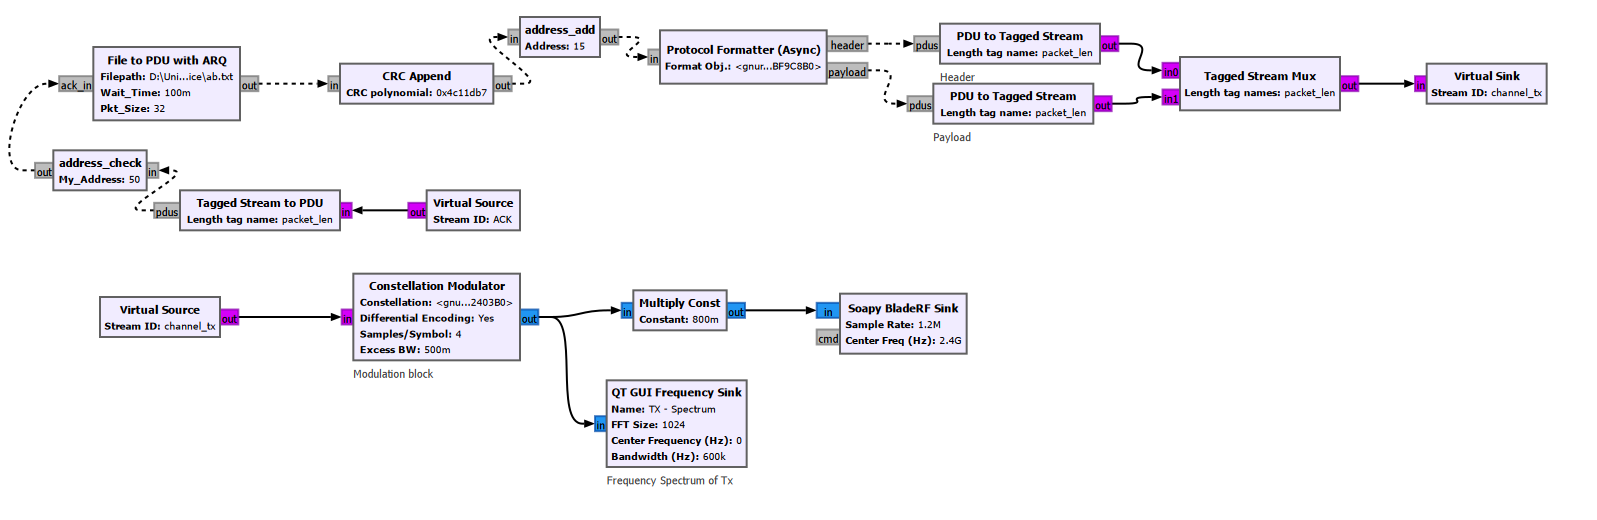
\includegraphics[width=1\linewidth]{tx1}
		\caption{Message Transmitter Block}
		\label{fig:tx1}
	\end{figure}
	
	\end{frame}

	\begin{frame}{Acknowledgement Receiver Block}
	
		\begin{figure}
			\centering
			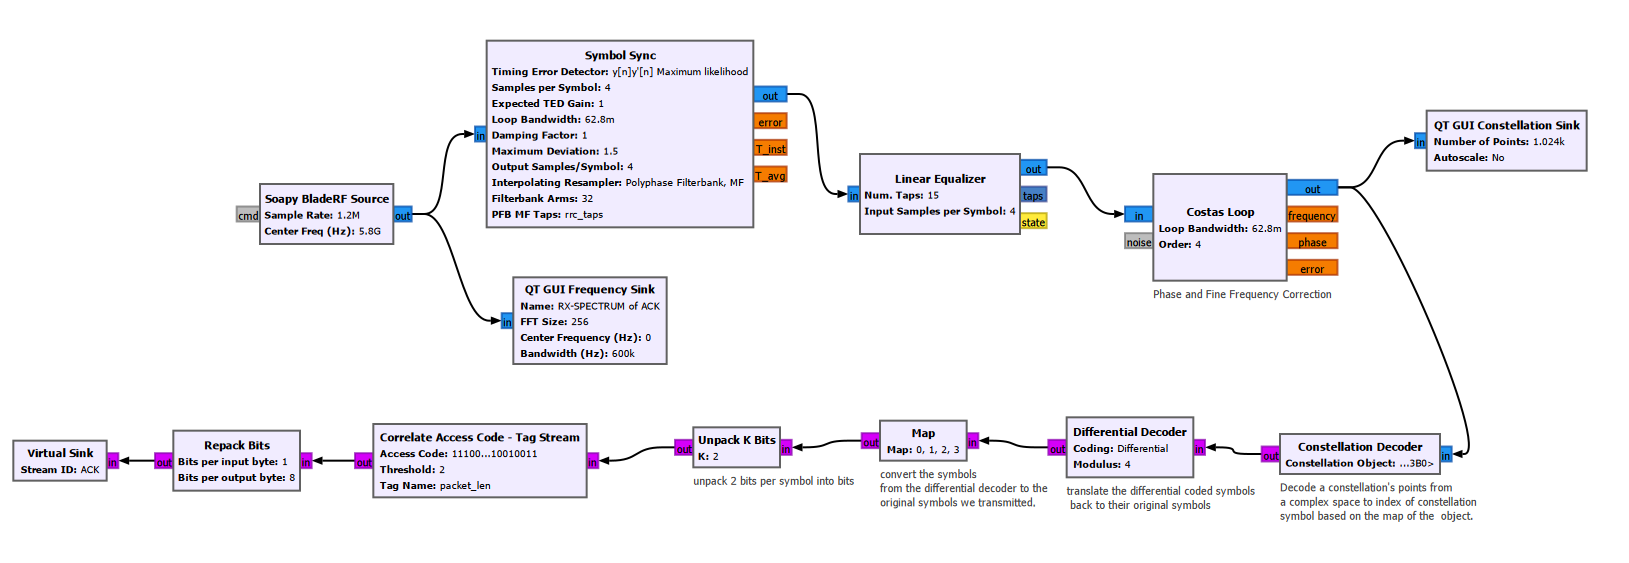
\includegraphics[width=1\linewidth]{tx2}
			\caption{Acknowledgement Receiver Block}
			\label{fig:tx2}
		\end{figure}
		
	\end{frame}
	
	\begin{frame}{Blocks \& Descriptions}
		Message Transmitter Block
	\begin{itemize}
		\item \textbf{Message Source:\footnote{Custom Python Block}\label{fn:1}} 
		Custom Python block that reads the input file/message, segments it into packets, 
		and prepares data for transmission. It also processes acknowledgment (ACK) messages from the receiver.
		
		\item \textbf{CRC Append:} 
		Adds a Cyclic Redundancy Check (CRC) code to each packet, enabling error detection 
		at the receiver and ensuring corrupted messages are discarded.
		
		\item \textbf{Protocol Formatter:} 
		Frames each packet with a header (containing sync word, addressing, etc.) and payload, 
		ensuring proper synchronization and identification.
		
	\item \textbf{Address Add:$^1$} Add the destination address to the frame
			\end{itemize}
	\end{frame}
	
		\begin{frame}{Blocks \& Descriptions (Contd...)}
		\begin{itemize}
				\item \textbf{PDU $\leftrightarrow$ Tagged Stream Conversion:} 
			Converts packet-based data (PDUs) into tagged streams for modulation, and back again 
			at the receiver. This allows GNU Radio blocks to handle both continuous streams and discrete packets.
		\item \textbf{Stream Mux:} 
		Combines headers and payloads into a single stream for transmission.
		
		\item \textbf{QPSK Modulator:} 
		Maps digital bits into complex QPSK symbols for RF transmission, providing 
		bandwidth efficiency and robustness.
		
	\end{itemize}
	\vspace{0.5cm}
	Acknowledgement Receiver Block
	\begin{itemize}
		    \item \textbf{Symbol Synchronization:} 
		Aligns the received signal samples with symbol timing to reduce inter-symbol interference.
		
		\item \textbf{Linear Equalizer:} 
		Compensates for channel distortions and multipath effects, improving signal quality.
		
		
	
	\end{itemize}
\end{frame}
\begin{frame}{Blocks \& Descriptions (Contd...)}
	\begin{itemize}
	\item \textbf{Costas Loop:} 
	Corrects carrier frequency and phase offsets in the received signal, enabling proper demodulation.
	
			\item \textbf{QPSK Decoder:} 
		Converts received QPSK symbols back into digital bits.
		
		\item \textbf{Differential Decoder:} 
		Removes phase ambiguity introduced during modulation/demodulation.
		
		\item \textbf{Bit Mapping + Unpack/Repack:} 
		Reconstructs the bitstream into meaningful packets, ready for higher-layer processing.
	\item \textbf{Address Check:$^1$} Checking whether the destination address is correct and passing though it.
		
		\item \textbf{ACK Feedback Path:$^1$} 
		Ensures reliable delivery by informing the transmitter whether a message was correctly received.
		
	\end{itemize}
	\end{frame}
	\section{Receiver}
	
		\begin{frame}
		\begin{center}
			{\Huge Receiver}
		\end{center}
	\end{frame}
	\begin{frame}{Message Receiver Block}

	\begin{figure}
		\centering
		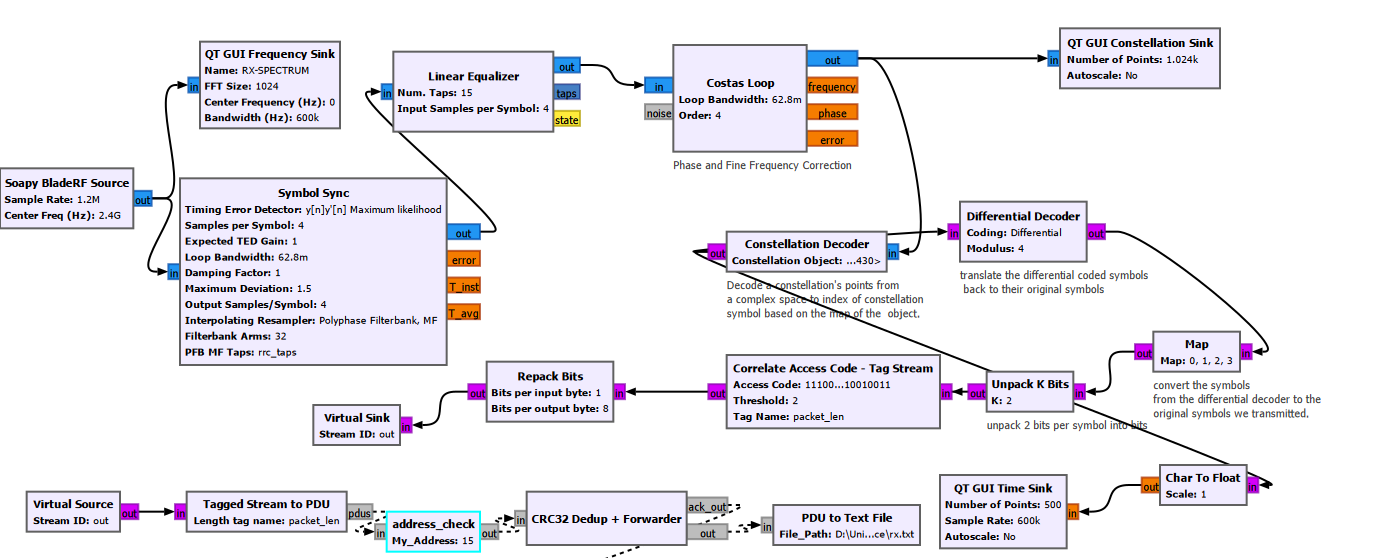
\includegraphics[width=1\linewidth]{rx1}
		\caption{Message Receiver Block Diagram}
		\label{fig:rx1}
	\end{figure}
	
	\end{frame}
	\begin{frame}{Acknowledgement Transmitter Block}

	\begin{figure}
		\centering
		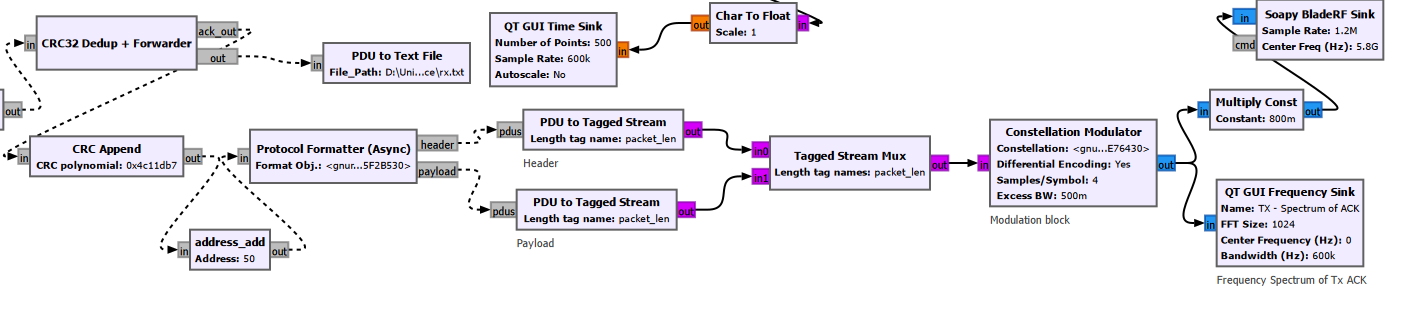
\includegraphics[width=1\linewidth]{rx2}
		\caption{Acknowledgement Transmitter Block}
		\label{fig:rx2}
	\end{figure}
		Other than blocks in transmitter,  we only used,
	\begin{itemize}
		\item \textbf{CRC 32 Dedup + Forwarder:}$^1$ Receives packets, checks their CRC32 for integrity, forwards the payload only if it’s not a duplicate, and always sends an acknowledgment (ACK) for valid packets. Essentially, it acts as a CRC validator, deduplicator, and forwarder.
	\end{itemize}
	\end{frame}
	
	
\section{Selected Methodologies}
	\begin{frame}
	\begin{center}
		{\Huge Selected Methodologies}
	\end{center}
\end{frame}
\begin{frame}{Frame structure}

\begin{figure}[H]
	\centering
	% Resize to fit page width
	\resizebox{0.9\textwidth}{!}{%
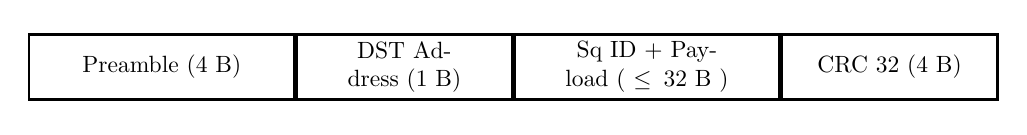
\begin{tikzpicture}[scale=0.85,transform shape]
	% Paths, nodes and wires:
	\node[shape=rectangle, draw, line width=1pt, minimum width=3.965cm, minimum height=0.965cm] at (-13, 7.5){} node[anchor=center, align=center, text width=3.577cm, inner sep=6pt] at (-13, 7.5){Preamble (4 B)};
	\node[shape=rectangle, draw, line width=1pt, minimum width=3.215cm, minimum height=0.965cm] at (-9.375, 7.5){} node[anchor=center, align=center, text width=2.827cm, inner sep=6pt] at (-9.375, 7.5){DST Address (1 B)};
	\node[shape=rectangle, draw, line width=1pt, minimum width=3.965cm, minimum height=0.965cm] at (-5.75, 7.5){} node[anchor=center, align=center, text width=3.577cm, inner sep=6pt] at (-5.75, 7.5){Sq ID + Payload ( $\le32$ B )};
	\node[shape=rectangle, draw, line width=1pt, minimum width=3.215cm, minimum height=0.965cm] at (-2.125, 7.5){} node[anchor=center, align=center, text width=2.827cm, inner sep=6pt] at (-2.125, 7.5){CRC 32 (4 B)};
\end{tikzpicture}
}


\caption{Message Frame}
\end{figure}

\begin{figure}[H]
	\centering
	% Resize to fit page width
	\resizebox{0.9\textwidth}{!}{%
		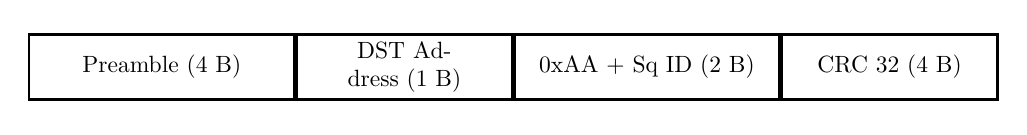
\begin{tikzpicture}[transform shape, scale=0.85]
			% Paths, nodes and wires:
			\node[shape=rectangle, draw, line width=1pt, minimum width=3.965cm, minimum height=0.965cm] at (-13, 7.5){} node[anchor=center, align=center, text width=3.577cm, inner sep=6pt] at (-13, 7.5){Preamble (4 B)};
			\node[shape=rectangle, draw, line width=1pt, minimum width=3.215cm, minimum height=0.965cm] at (-9.375, 7.5){} node[anchor=center, align=center, text width=2.827cm, inner sep=6pt] at (-9.375, 7.5){DST Address (1 B)};
			\node[shape=rectangle, draw, line width=1pt, minimum width=3.965cm, minimum height=0.965cm] at (-5.75, 7.5){} node[anchor=center, align=center, text width=3.577cm, inner sep=6pt] at (-5.75, 7.5){0xAA + Sq ID (2 B)};
			\node[shape=rectangle, draw, line width=1pt, minimum width=3.215cm, minimum height=0.965cm] at (-2.125, 7.5){} node[anchor=center, align=center, text width=2.827cm, inner sep=6pt] at (-2.125, 7.5){CRC 32 (4 B)};
		\end{tikzpicture}
		
	}
\caption{Acknowledgement Frame}
\end{figure}
Maximum text file size\footnote{For this frame design $N=31$. Therefore, Maximum text file size = $7905$ Bytes.} =$ (2^{8}-1)\times N$ Bytes, 
where $N$ is the number of data bytes in payload.\\

\end{frame}
	\begin{frame}{ARQ Mechanism}
		
		We are using a \textbf{Stop-and-Wait ARQ} system:
		
		\begin{description}
			\item[Step 1:] Each frame carries an \textbf{address}.
			\item[Step 2:] The receiver checks the \textbf{address}.
			\item[Step 3:] If correct, it sends an \textbf{ACK} back.
			\item[Step 4:] The sender waits for the ACK. If it is missing, the sender \textbf{retransmits} the same frame.
		\end{description}\centering
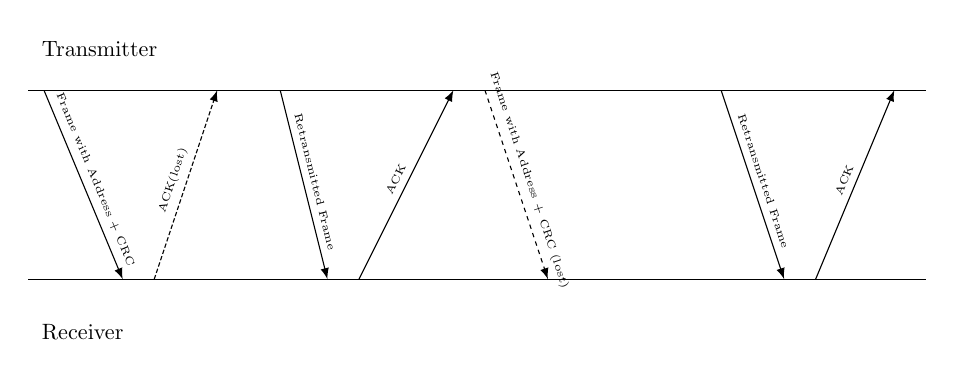
\begin{tikzpicture}[scale=0.8, transform shape]
	% Paths, nodes and wires:
	\draw (-13, 5) -- (1.25, 5) ;
	\draw (-13, 2) -- (1.25, 2);
	\draw[-latex] (-12.75, 5) -- (-11.5, 2) node[midway, above, sloped] {\tiny Frame with Address + CRC};
	\draw[dash pattern={on 1.6pt off 0.8pt}, -latex] (-11, 2) -- (-10, 5) node[midway, above, sloped] {\tiny ACK(lost)};
	\draw[-latex] (-9.0, 5) -- (-8.25, 2)node[midway, above, sloped] {\tiny Retransmitted Frame};
	\draw[ -latex] (-7.75, 2) -- (-6.25, 5)node[midway, above, sloped] {\tiny ACK};
	\draw[dash pattern={on 1.6pt off 1.6pt}, -latex] (-5.75, 5) -- (-4.75, 2)node[midway, above, sloped] {\tiny Frame with Address + CRC (lost)};
	\draw[-latex] (-2, 5) -- (-1, 2)node[midway, above, sloped] {\tiny Retransmitted Frame};
	\draw[-latex] (-0.5, 2) -- (0.75, 5)node[midway, above, sloped] {\tiny ACK};;
	\node[shape=rectangle, minimum width=1.965cm, minimum height=0.465cm] at (-12, 5.75){} node[anchor=north west, align=left, text width=1.577cm, inner sep=6pt] at (-13, 6){Transmitter};
	\node[shape=rectangle, minimum width=2.215cm, minimum height=0.715cm] at (-11.875, 1.125){} node[anchor=north west, align=left, text width=1.827cm, inner sep=6pt] at (-13, 1.5){Receiver};
\end{tikzpicture}
	\end{frame}
	
	\begin{frame}[fragile]{How ARQ Mechanism Visible in GNU Radio?}

		\tiny
		\begin{verbatim}
			

	[CRC32] OK (Packet 20)
	[Forward] Packet 20 duplicate, not forwarded
	[FilePDU] Timeout waiting for ACK of 0x15, retrying...
	[FilePDU] Packet 0x15 sent (try 2)
	[CRC32] OK (Packet 21)
	[Forward] UTF-8 decode error: 'charmap' codec can't encode character '\u2192' in
	position 20: character maps to <undefined>
	[TextFile] Wrote 31 chars to D:\University\Semester 3\EN2130\gnupractice\rx.txt
	[FilePDU] Timeout waiting for ACK of 0x15, retrying...
	[FilePDU] Packet 0x15 sent (try 3)
	[CRC32] OK (Packet 21)
	[Forward] Packet 21 duplicate, not forwarded
	[FilePDU] ACK received for packet 0x15
	[FilePDU] Packet 0x16 sent (try 1)
	[CRC32] OK (Packet 21)
	[Forward] Packet 21 duplicate, not forwarded
	[FilePDU] Timeout waiting for ACK of 0x16, retrying...
	[FilePDU] Packet 0x16 sent (try 2)
	[CRC32] OK (Packet 22)
	[Forward] UTF-8 decode error: 'charmap' codec can't encode character '\u2192' in
	position 20: character maps to <undefined>
	[TextFile] Wrote 7 chars to D:\University\Semester 3\EN2130\gnupractice\rx.txt
	[FilePDU] Timeout waiting for ACK of 0x16, retrying...
	[FilePDU] Packet 0x16 sent (try 3)
	[CRC32] OK (Packet 22)
	[Forward] Packet 22 duplicate, not forwarded
	[FilePDU] ACK received for packet 0x16
		\end{verbatim}
	
		
	\end{frame}
\begin{frame}{QPSK Modulation}
	\begin{itemize}
		\item \textbf{Quadrature Phase Shift Keying (QPSK)} is used as the modulation scheme.
		\item Each symbol carries \textbf{2 bits}, mapped to one of four constellation points.
		\item Constellation points: $(\pm 1, \pm 1)$ with Gray coding to minimize bit errors.
		\item \textbf{Advantages:}
		\begin{itemize}
			\item Bandwidth efficient (2 bits/symbol).
			\item Robust against noise compared to higher-order modulations.
		\end{itemize}
		\item Symbol synchronization is used to correctly recover symbols at the receiver.
	\end{itemize}
\end{frame}

	\begin{frame}{Simulation Results}

	\begin{figure}
		\centering
		\includegraphics[height=0.3\textheight]{"C:/Users/ASUS TUF X506H/Pictures/Screenshots/Screenshot (77)"}
		\caption{Constellation Diagrams}
		\label{fig:screenshot-77}
	\end{figure}
	
	\begin{figure}
		\centering
		\includegraphics[width=1\textwidth]{"C:/Users/ASUS TUF X506H/Pictures/Screenshots/Screenshot 2025-09-16 095607"}
		\caption{Frequency Spectrum}
		\label{fig:screenshot-2025-09-16-095607}
	\end{figure}
	
	
	\end{frame}

	
	\section*{Conclusion}
	\begin{frame}{References}
		
		\begin{thebibliography}{1}
			
			\bibitem{1}
			GNU Radio, ``Tutorials,'' GNU Radio Wiki. [Online]. Available: \url{https://wiki.gnuradio.org/index.php/Tutorials}. [Accessed: Sep. 14, 2025].
			
		\end{thebibliography}
	\end{frame}
	
	\begin{frame}
		\begin{center}
			{\Huge Thank You!}
		\end{center}
	\end{frame}
	
\end{document}
